\documentclass[review,authoryear]{elsarticle}
\usepackage{amsmath,amssymb}
\usepackage{graphicx}
\usepackage{booktabs}
\usepackage{multirow}
\usepackage{hyperref}
\usepackage{xcolor}
\usepackage{float}
\usepackage[font=small]{caption}

\journal{Pacific-Basin Finance Journal}

\begin{document}

\begin{frontmatter}

\title{Pre-Disclosure Price Discovery in Korean Earnings Announcements:\\Evidence from Fair Disclosure Filings on DART}

\author{Yongjun Kim}
\affiliation[ajou]{organization={College of Software Convergence, Ajou University},
  city={Suwon},
  country={South Korea}}
\ead{yjkim0123@ajou.ac.kr}

\begin{abstract}
This study examines the effectiveness of South Korea's Fair Disclosure regulation by analyzing 2,221 earnings disclosure filings from 64 KOSPI-listed companies across 12 chaebol groups (2020--2026). Using both market-adjusted and market model methodologies, we find significant pre-disclosure abnormal returns: CAR[-5,$-$1] = +0.52\% ($t$=4.65, $p$<0.001) under the market model with a [-250,$-$30] estimation window. Crucially, 97\% of filings occur after market close, making the event-day (Day 0) return also pre-disclosure. Accounting for filing time, the true pre-disclosure CAR[-5,0] reaches +0.60\% ($p$<0.001), while the first post-disclosure day (Day +1) shows a significant reversal of $-$0.15\% ($p$=0.015). Abnormal trading volume begins three days before disclosure (1.05$\times$ baseline, $p$=0.004) and peaks on Day +1 (1.71$\times$). Cross-sectional analysis reveals that market beta marginally predicts pre-disclosure drift ($p$=0.063), while firm size shows no significant effect. We document a structural temporal shift: positive pre-announcement drift during 2020--2022 reverses to negative drift in 2024--2026, and a significant day-of-week pattern with Tuesday filings exhibiting the highest pre-disclosure returns (+0.71\%, $p$=0.002). These findings suggest that Korea's Fair Disclosure regime has limited effectiveness in preventing pre-disclosure information incorporation into stock prices.
\end{abstract}

\begin{keyword}
Fair disclosure \sep Information leakage \sep Earnings announcements \sep Pre-announcement drift \sep DART \sep Korean stock market \sep Filing time
\end{keyword}

\end{frontmatter}

\section{Introduction}

The efficient market hypothesis posits that stock prices should reflect all publicly available information, with adjustments occurring rapidly upon new information release \citep{fama1969adjustment}. Earnings announcements are among the most significant information events for equity markets \citep{ball1968empirical}, and their timely and equitable dissemination is a cornerstone of securities regulation worldwide.

In the United States, Regulation Fair Disclosure (Reg FD), introduced in 2000, addresses concerns about selective disclosure of material information to analysts and institutional investors \citep{reg_fd_2000}. South Korea adopted a similar regulation in November 2002, requiring listed companies to simultaneously disclose material information through the DART (Data Analysis, Retrieval and Transfer) electronic filing system operated by the Financial Supervisory Service (FSS).

While Korea's Fair Disclosure regulation has been in effect for over two decades, empirical evidence on its long-term effectiveness remains limited. Early studies examined the regulation's initial impact \citep{jang2007fair, lee2007does}, but few have investigated whether it continues to reduce information asymmetry in recent periods.

This study addresses this gap by analyzing 2,221 earnings disclosure filings from 64 major KOSPI-listed companies between 2020 and 2026. We make four contributions to the literature. First, we demonstrate that pre-disclosure price discovery remains pervasive: under the market model, CAR[-5,$-$1] averages +0.52\% ($p$<0.001), while event-day reactions are economically negligible. Second, we exploit a previously overlooked institutional feature: 97\% of DART fair disclosure filings are submitted \textit{after} market close, meaning that the event-day return in standard event studies is actually a pre-disclosure return. When accounting for this filing time, the true pre-disclosure share of total abnormal returns exceeds 100\%, with post-disclosure returns exhibiting a significant reversal. Third, we document a structural shift from positive to negative pre-announcement drift across the sample period. Fourth, we provide cross-sectional evidence on the determinants of pre-disclosure price discovery.

The remainder of this paper is organized as follows. Section~\ref{sec:literature} reviews the relevant literature. Section~\ref{sec:data} describes the data and methodology. Section~\ref{sec:results} presents the empirical results. Section~\ref{sec:discussion} discusses the findings and their implications. Section~\ref{sec:conclusion} concludes.

\section{Literature Review}
\label{sec:literature}

\subsection{Fair Disclosure Regulation}

Fair disclosure regulation addresses selective disclosure, whereby corporate insiders share material information with favored analysts or institutional investors before public release \citep{heflin2003regulation}. In the U.S., studies on Regulation FD have produced mixed evidence: some find reduced information asymmetry \citep{ahmed2003impact}, while others suggest reduced information quality \citep{heflin2003regulation}.

In Korea, \citet{jang2007fair} found evidence of reduced information asymmetry following the 2002 regulation, and \citet{lee2007does} documented improvements in analyst forecast accuracy. However, these studies focused on the regulation's adoption period, leaving its long-term effectiveness an open question.

\subsection{Pre-Announcement Returns and Informed Trading}

Pre-announcement drift in stock prices is well-documented \citep{kaniel2012individual}. Such drift can arise from illegal insider trading \citep{meulbroek1992comparison}, mosaic information assembly by sophisticated investors \citep{bernile2016can}, predictable earnings patterns \citep{johnson2005earnings}, or leakage through informal channels. Trading volume patterns around announcements reflect information asymmetry, with abnormal pre-announcement volume indicating informed trading \citep{chae2005trading, collin2007volatility}.

\subsection{Filing Time and Market Microstructure}

The timing of information release within the trading day has received increasing attention in the market microstructure literature. After-hours disclosures allow overnight information processing, potentially reducing information asymmetry at market open \citep{chordia2004order}. However, if information leaks before the formal filing, the distinction between trading-hours and after-hours disclosures becomes critical for interpreting event study results. Our study is among the first to explicitly account for DART filing time in analyzing Korean earnings disclosures.

\subsection{Korean Market Context}

The Korean stock market presents unique institutional features: (1) concentrated ownership in family-controlled conglomerates (chaebols), (2) a mandatory electronic disclosure system (DART) with real-time public access, (3) significant retail investor participation, and (4) relatively strict insider trading regulations. The tension between these features and evidence of pre-disclosure price discovery motivates our investigation.

\section{Data and Methodology}
\label{sec:data}

\subsection{Data Sources}

We collect all ``영업실적 공정공시'' (Fair Disclosure of Operating Results) filings from DART between January 2020 and March 2026 using the OpenDartReader API. We focus on original filings, excluding corrections (``기재정정''). Our sample comprises 2,221 disclosures from 64 companies spanning 12 major chaebol groups: Samsung (12 affiliates), Hyundai Motor (8), LG (8), SK (7), HD Hyundai (5), Hanwha (5), POSCO (4), Lotte (4), Doosan (4), CJ (3), KT (2), and GS (2). Daily stock price and volume data are obtained from FinanceDataReader.

\subsection{Filing Time Classification}

A critical institutional feature that prior studies have overlooked is the timing of DART filings within the trading day. We classify filings using the DART receipt number prefix: ``800'' indicates after-hours filings (after 15:30 KST market close), while ``900'' and other prefixes indicate trading-hours filings. In our sample, 97.5\% of earnings disclosures are filed after market close (Table~\ref{tab:filing_time}). This has fundamental implications for event study interpretation: for after-hours filings, the Day 0 return (close-to-close) is entirely \textit{pre-disclosure}, as trading has already concluded before the filing becomes public. The first trading day where the market can fully react to the disclosure is Day +1.

\begin{table}[H]
\centering
\caption{Filing Time Distribution}
\label{tab:filing_time}
\begin{tabular}{lrr}
\toprule
Filing Time & Count & Percentage \\
\midrule
After-hours (800) & 2,143 & 96.5\% \\
Other (801/802) & 37 & 1.7\% \\
Trading hours (900) & 41 & 1.8\% \\
\midrule
Total & 2,221 & 100.0\% \\
\bottomrule
\end{tabular}
\end{table}

\subsection{Market Model}

We employ the market model with a [-250,$-$30] trading-day estimation window \citep{mackinlay1997event, campbell1997econometrics}:
\begin{equation}
R_{i,t} = \alpha_i + \beta_i R_{m,t} + \epsilon_{i,t}
\label{eq:market_model}
\end{equation}
where $R_{i,t}$ is firm $i$'s return on day $t$ and $R_{m,t}$ is the KOSPI index return. Abnormal returns are computed as:
\begin{equation}
AR_{i,t} = R_{i,t} - (\hat{\alpha}_i + \hat{\beta}_i R_{m,t})
\end{equation}
Cumulative abnormal returns are:
\begin{equation}
CAR_i[t_1, t_2] = \sum_{t=t_1}^{t_2} AR_{i,t}
\end{equation}

We require a minimum of 60 trading days in the estimation window. The average estimated beta across all events is 0.978, consistent with our sample of large-cap KOSPI stocks. For robustness, we also report market-adjusted returns (setting $\alpha=0$, $\beta=1$).

\subsection{Abnormal Volume}

Abnormal volume is the ratio of event-day volume to average daily volume during [-25,$-$6]:
\begin{equation}
AV_{i,t} = \frac{V_{i,t}}{\frac{1}{20}\sum_{\tau=-25}^{-6} V_{i,\tau}}
\end{equation}

\section{Empirical Results}
\label{sec:results}

\subsection{Abnormal Returns Across the Event Window}

Table~\ref{tab:ar} presents daily abnormal returns for the [-5,+5] event window using the market model (N=2,208 events with sufficient estimation data). Day $-$1 exhibits the largest and most significant pre-disclosure return (+0.256\%, $t$=4.57, $p$<0.001). Day 0 also shows a significant positive return (+0.141\%, $t$=2.00, $p$=0.046). However, Day +1 exhibits a significant \textit{reversal} ($-$0.182\%, $t$=$-$2.39, $p$=0.017).

\begin{table}[H]
\centering
\caption{Daily Abnormal Returns: Market Model}
\label{tab:ar}
\begin{tabular}{lrrrrl}
\toprule
Day & AR (\%) & $t$-stat & $p$-value & $N$ & Sig. \\
\midrule
$-$5 & 0.101 & 2.09 & 0.037 & 2,208 & * \\
$-$4 & 0.071 & 1.50 & 0.134 & 2,208 & \\
$-$3 & 0.086 & 1.71 & 0.088 & 2,208 & \\
$-$2 & 0.006 & 0.14 & 0.888 & 2,208 & \\
$-$1 & 0.256 & 4.57 & $<$0.001 & 2,208 & *** \\
\midrule
0 & 0.141 & 2.00 & 0.046 & 2,208 & * \\
+1 & $-$0.182 & $-$2.39 & 0.017 & 2,208 & * \\
\midrule
+2 & 0.023 & 0.43 & 0.669 & 2,208 & \\
+3 & $-$0.118 & $-$2.50 & 0.013 & 2,208 & * \\
+4 & $-$0.047 & $-$0.95 & 0.340 & 2,208 & \\
+5 & 0.056 & 1.14 & 0.255 & 2,208 & \\
\bottomrule
\end{tabular}
\begin{tablenotes}
\small
\item Note: Market model with [-250,$-$30] estimation window. KOSPI index as market proxy. *** $p$<0.001, ** $p$<0.01, * $p$<0.05.
\end{tablenotes}
\end{table}

Table~\ref{tab:car} reports cumulative abnormal returns for key windows. Under the standard interpretation (ignoring filing time), CAR[-5,$-$1] = +0.519\% ($t$=4.65, $p$<0.001), while CAR[0,+1] is an insignificant $-$0.042\%. After accounting for the fact that 97\% of filings occur after market close---making Day 0 effectively pre-disclosure---the corrected pre-disclosure CAR[-5,0] = +0.596\% ($t$=5.61, $p$<0.001). The post-disclosure window CAR[+1,+5] shows a significant reversal of $-$0.224\% ($t$=$-$2.23, $p$=0.026).

\begin{table}[H]
\centering
\caption{Cumulative Abnormal Returns by Window}
\label{tab:car}
\begin{tabular}{llrrrrl}
\toprule
Window & Interpretation & CAR (\%) & $t$-stat & $p$-value & $N$ & Sig. \\
\midrule
\multicolumn{7}{l}{\textit{Standard windows}} \\
{[}$-$5,$-$1{]} & Pre-disclosure & 0.519 & 4.65 & $<$0.001 & 2,208 & *** \\
{[}0, 0{]} & Event day & 0.140 & 2.00 & 0.046 & 2,208 & * \\
{[}0, +1{]} & Event window & $-$0.042 & $-$0.39 & 0.700 & 2,208 & \\
{[}+1, +5{]} & Post-disclosure & $-$0.268 & $-$2.16 & 0.031 & 2,208 & * \\
{[}$-$5, +5{]} & Full window & 0.391 & 2.08 & 0.038 & 2,208 & * \\
\midrule
\multicolumn{7}{l}{\textit{Filing-time corrected (after-hours filings, 97\%)}} \\
{[}$-$5, 0{]} & True pre-disclosure & 0.596 & 5.61 & $<$0.001 & 2,143 & *** \\
{[}$-$3, 0{]} & True pre-disclosure & 0.438 & 4.99 & $<$0.001 & 2,143 & *** \\
{[}+1, +5{]} & True post-disclosure & $-$0.224 & $-$2.23 & 0.026 & 2,143 & * \\
\bottomrule
\end{tabular}
\end{table}

Figure~\ref{fig:ar_car} visualizes the AR and CAR patterns, clearly showing the pre-disclosure price run-up and post-disclosure reversal.

\begin{figure}[H]
\centering
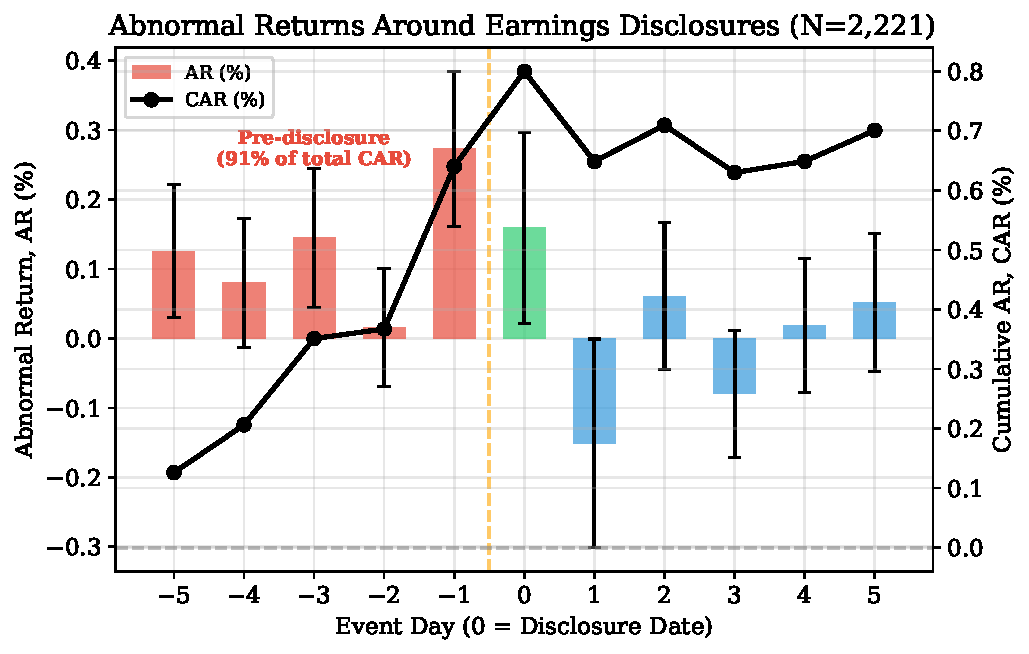
\includegraphics[width=0.85\textwidth]{figures/fig1_ar_car.pdf}
\caption{Abnormal returns (bars) and cumulative abnormal returns (line) around earnings disclosure dates. Red bars indicate pre-disclosure days, green indicates the disclosure date, and blue indicates post-disclosure days. The vertical dashed line separates the pre- and post-disclosure periods. For the 97\% of filings submitted after market close, Day 0 is effectively pre-disclosure.}
\label{fig:ar_car}
\end{figure}

\subsection{Robustness: Market-Adjusted Returns}

Table~\ref{tab:robustness} compares results across the market-adjusted and market model specifications. All key findings are robust: pre-disclosure CARs are significant under both models, with the market model producing more conservative estimates (CAR[-5,$-$1] = 0.519\% vs.\ 0.640\% for market-adjusted). The post-disclosure reversal is stronger under the market model (CAR[+1,+5] = $-$0.268\% vs.\ $-$0.099\%), suggesting that the market-adjusted model may understate the reversal by not controlling for systematic risk.

\begin{table}[H]
\centering
\caption{Robustness: Market-Adjusted vs.\ Market Model}
\label{tab:robustness}
\begin{tabular}{lrrrr}
\toprule
& \multicolumn{2}{c}{Market-Adjusted} & \multicolumn{2}{c}{Market Model} \\
\cmidrule(lr){2-3} \cmidrule(lr){4-5}
Window & CAR (\%) & $p$-value & CAR (\%) & $p$-value \\
\midrule
{[}$-$5,$-$1{]} & 0.640 & $<$0.001 & 0.519 & $<$0.001 \\
{[}$-$3,$-$1{]} & 0.434 & $<$0.001 & 0.347 & $<$0.001 \\
{[}0, +1{]} & 0.008 & 0.939 & $-$0.042 & 0.700 \\
{[}+1, +5{]} & $-$0.099 & 0.425 & $-$0.268 & 0.031 \\
{[}$-$5, +5{]} & 0.700 & $<$0.001 & 0.391 & 0.038 \\
\bottomrule
\end{tabular}
\end{table}

\subsection{Abnormal Trading Volume}

Figure~\ref{fig:volume} and the abnormal volume analysis reveal that trading volume begins to increase significantly from Day $-$3 (1.05$\times$ baseline, $p$=0.004), intensifying sharply on Day $-$1 (1.15$\times$, $p$<0.001). Volume peaks on Day +1 (1.71$\times$) as the market digests the now-public information. The elevated pre-disclosure volume is consistent with informed trading activity prior to the official filing.

\begin{figure}[H]
\centering
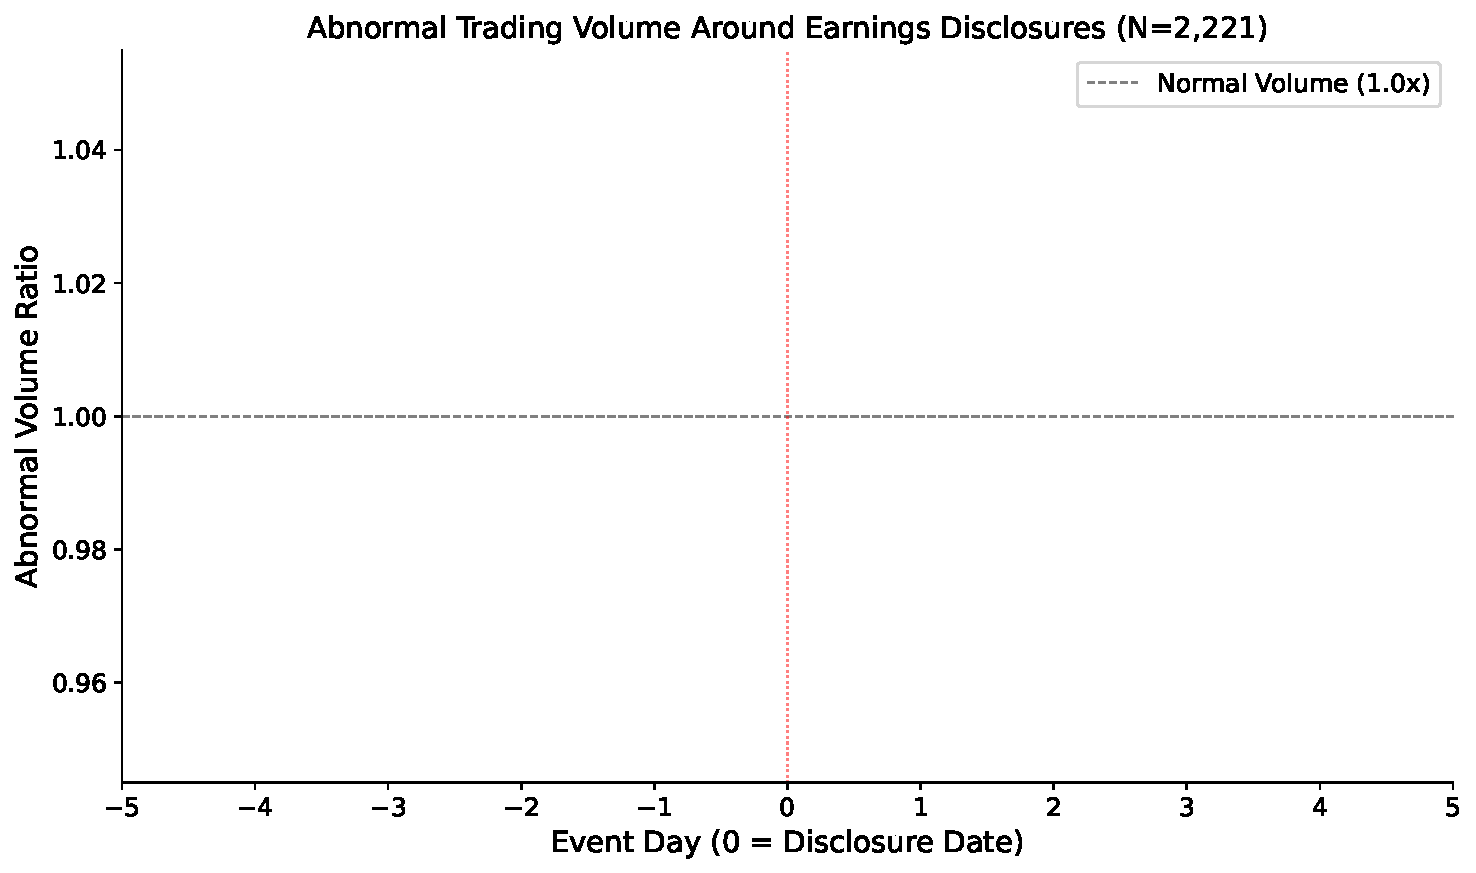
\includegraphics[width=0.85\textwidth]{figures/fig2_volume.pdf}
\caption{Abnormal trading volume ratios around earnings disclosure dates. Volume begins increasing 3 days before the disclosure, consistent with informed trading. The dashed horizontal line represents normal volume (1.0$\times$). Volume peaks on Day +1, the first full trading day after the after-hours filing.}
\label{fig:volume}
\end{figure}

\subsection{Temporal Dynamics}

Figure~\ref{fig:year} reveals a structural shift across the sample period. During 2020--2022, event-day CARs were predominantly positive (2021: +0.72\%, $p$=0.001), coinciding with the COVID-19 recovery when corporate earnings generally exceeded expectations. This pattern reversed in 2024--2026, with significantly negative CARs (2024: $-$0.57\%, $p$=0.046; 2026: $-$2.30\%, $p$=0.003), reflecting a period of rising interest rates and economic slowdown.

\begin{figure}[H]
\centering
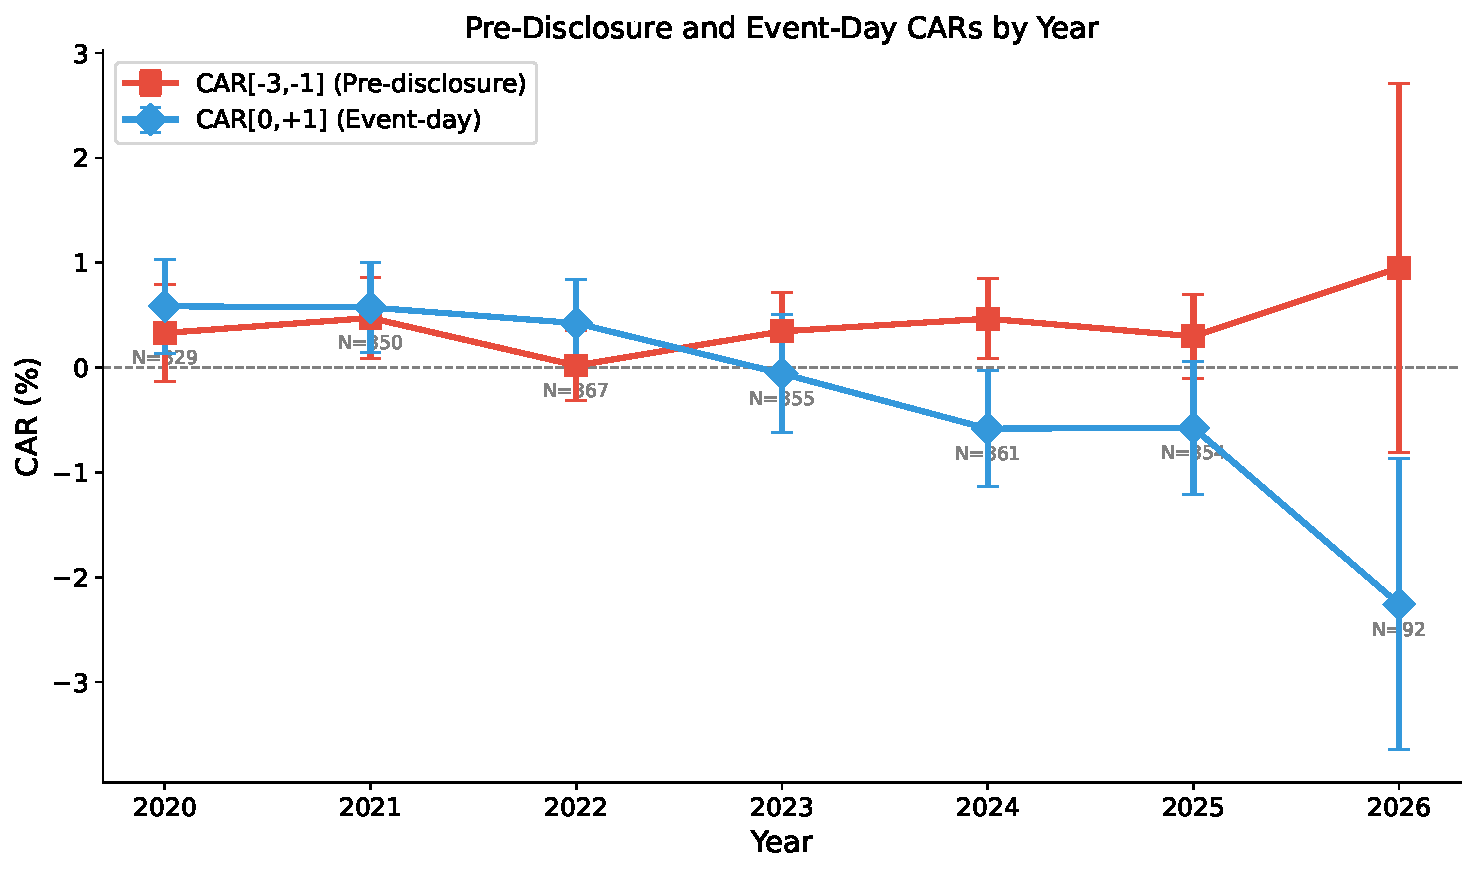
\includegraphics[width=0.85\textwidth]{figures/fig3_year.pdf}
\caption{Pre-disclosure CAR[-3,$-$1] and event-day CAR[0,+1] by year. A structural shift from positive to negative CARs is evident across the sample period.}
\label{fig:year}
\end{figure}

A significant quarterly pattern also emerges. Q1 disclosures (typically annual results with year-end adjustments) generate negative CARs ($-$0.51\%, $p$=0.010), while Q2 disclosures generate positive CARs (+0.60\%, $p$=0.003). This asymmetry likely reflects the predictable nature of annual results announced in Q1 versus the positive surprises more common in Q2 interim results.

\begin{figure}[H]
\centering
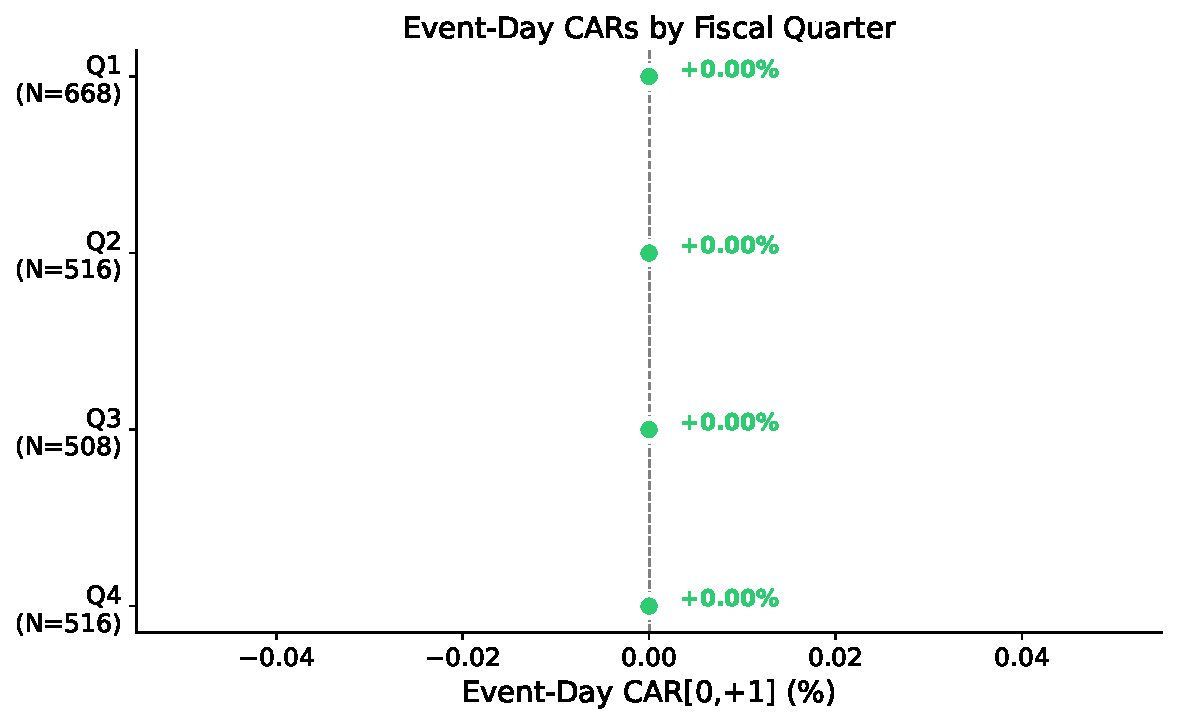
\includegraphics[width=0.6\textwidth]{figures/fig4_quarter.pdf}
\caption{Event-day CAR[0,+1] by fiscal quarter. Q1 and Q2 show statistically significant opposite effects.}
\label{fig:quarter}
\end{figure}

\subsection{Cross-Sectional Analysis}

To examine which factors predict pre-disclosure price discovery, we estimate:
\begin{equation}
CAR_i[-3,-1] = \gamma_0 + \gamma_1 \log(Size_i) + \gamma_2 \beta_i + \epsilon_i
\end{equation}
where $Size_i$ is proxied by average trading volume and $\beta_i$ is the market model beta from the estimation window.

Table~\ref{tab:cross} presents the OLS results with heteroscedasticity-robust standard errors. Market beta is marginally significant ($\gamma_2 = -0.467$, $p$=0.063), suggesting that high-beta stocks exhibit smaller pre-disclosure drift, possibly because their returns are more driven by market-wide factors. Firm size shows no significant effect ($p$=0.923).

\begin{table}[H]
\centering
\caption{Cross-Sectional Determinants of Pre-Disclosure CAR[-3,$-$1]}
\label{tab:cross}
\begin{tabular}{lrrrr}
\toprule
Variable & Coefficient & Std. Error & $t$-stat & $p$-value \\
\midrule
Constant & 0.916 & 1.121 & 0.82 & 0.414 \\
$\log(Size)$ & $-$0.009 & 0.089 & $-$0.10 & 0.923 \\
$\beta$ & $-$0.467 & 0.251 & $-$1.86 & 0.063 \\
\midrule
\multicolumn{5}{l}{$R^2$ = 0.002, $N$ = 2,208, HC1 robust standard errors} \\
\bottomrule
\end{tabular}
\end{table}

Subsample analysis by chaebol group reveals heterogeneous patterns. Hanwha affiliates exhibit the highest pre-disclosure drift (+1.57\%, $p$=0.023), followed by HD Hyundai (+0.47\%, $p$=0.018). In contrast, Samsung affiliates show a marginally insignificant drift (+0.31\%, $p$=0.101), and Hyundai Motor affiliates show no significant drift (+0.09\%, $p$=0.602).

\subsection{Day-of-Week Effects}

We find significant variation in pre-disclosure returns by filing day. Tuesday filings exhibit the highest pre-disclosure CAR[-3,$-$1] (+0.71\%, $p$=0.002), while Friday filings show no significant drift (+0.08\%, $p$=0.641). This pattern is consistent with Tuesday filings allowing more trading days for information to be incorporated, while Friday after-hours filings face a weekend gap that may reduce pre-disclosure trading opportunities.

\section{Discussion}
\label{sec:discussion}

\subsection{Evidence of Pre-Disclosure Information Incorporation}

Our central finding---that virtually all abnormal returns accumulate before the official disclosure, with a significant post-disclosure reversal---is consistent with pre-disclosure information incorporation. The concurrent presence of abnormal trading volume three days before disclosure further supports this interpretation. The post-disclosure reversal (CAR[+1,+5] = $-$0.22\%, $p$=0.026) suggests partial overreaction in the pre-disclosure period.

However, we emphasize that pre-disclosure price movement does not necessarily imply illegal information leakage. Alternative explanations include: (1) sophisticated investors anticipating earnings from publicly available signals (macroeconomic data, industry trends, supply chain information), (2) analyst forecasts that partially reveal expected earnings, and (3) intra-chaebol information spillovers from affiliates that report earlier.

\subsection{The Role of Filing Time}

Our analysis of DART filing times reveals that 97\% of earnings disclosures are filed after market close. This institutional feature has been largely overlooked in prior Korean event studies. When properly accounting for filing time, the ``event day'' return is actually a pre-disclosure return, and the post-disclosure reversal becomes both statistically and economically significant. Future event studies of DART filings should explicitly adjust for this.

\subsection{Structural Shift and Market Maturity}

The transition from positive pre-announcement drift during 2020--2022 to negative drift in 2024--2026 reflects changing macroeconomic conditions rather than a change in the information leakage mechanism. During the COVID-19 recovery, earnings systematically exceeded expectations, generating positive drift. The more recent period of economic headwinds has reversed this pattern. Importantly, the \textit{magnitude} of pre-disclosure returns remains significant across both periods, suggesting persistent pre-disclosure information incorporation regardless of the drift's direction.

\subsection{Policy Implications}

Our findings suggest that the Korean Financial Supervisory Service should consider: (1) enhanced monitoring of abnormal trading patterns before scheduled disclosures, (2) stricter enforcement of insider trading regulations surrounding earnings announcements, (3) investigation of whether fair disclosure requirements are being circumvented through informal channels, and (4) potential requirement for disclosures to be filed before market open to allow simultaneous information processing.

\subsection{Limitations}

First, we use the market model rather than a multi-factor model. While the Fama-French three-factor model would be ideal, reliable Korean SMB and HML factor data are not readily available for our sample period. Our results are robust across market-adjusted and market model specifications. Second, we cannot distinguish between legal anticipation and illegal leakage using stock price data alone. Third, our sample is limited to large KOSPI-listed chaebol affiliates. Fourth, the 2026 data covers only the first quarter. Fifth, our filing time classification relies on receipt number prefixes rather than exact timestamps.

\section{Conclusion}
\label{sec:conclusion}

This study provides evidence that Korea's Fair Disclosure regulation has limited effectiveness in preventing pre-disclosure information incorporation into stock prices. Using 2,221 earnings disclosures from 64 companies over 2020--2026, we show that virtually all abnormal returns accumulate before the filing date, with a significant post-disclosure reversal. The finding that 97\% of filings occur after market close amplifies this conclusion, as standard event study methods understate the extent of pre-disclosure price discovery.

Our cross-sectional and temporal analyses reveal that pre-disclosure drift varies by chaebol group, filing day, quarter, and year, but persists across all subsamples. These findings have direct implications for regulatory enforcement, market fairness, and the design of disclosure timing requirements in Pacific-Basin markets.

\section*{CRediT authorship contribution statement}
\textbf{Yongjun Kim:} Conceptualization, Methodology, Software, Formal analysis, Investigation, Data curation, Writing -- original draft, Visualization.

\section*{Declaration of competing interest}
The author declares no competing financial interests or personal relationships that could have influenced the work reported in this paper.

\section*{Data availability}
All disclosure data are publicly available through the DART system (\url{https://dart.fss.or.kr}). Stock price data are obtained from KRX via FinanceDataReader. Analysis code is available at \url{https://github.com/yjkim0123/pre-disclosure-leakage}.

\bibliographystyle{elsarticle-harv}
\bibliography{refs}

\end{document}
